%\subsection{Nodal bases and dual bases on multilevel spaces}
%\noindent\textbf{Nodal bases and dual bases on multilevel spaces}

Here each $\mathcal V_\ell$ consists of all piecewise linear (or bilinear)
functions with respect to the grid \eqref{grids} and \eqref{mn-ell}.
Each $\mathcal V_\ell $ has a set of basis functions:
$\phi_{i,j}^\ell\in \mathcal V_\ell$ satisfying:
\begin{equation}
\label{NodalBases-mul}
\mathbf\phi_{i,j}^\ell(x_p^\ell,y_q^\ell)=\delta_{(i,j), (p,q)} = 
\begin{cases}
1 \quad &\text{if} \quad (p,q) = (i,j), \\
0 \quad &{\text{if}} \quad (p,q)\neq (i,j).
\end{cases}
\end{equation}
\begin{figure}[!ht]
\begin{center}
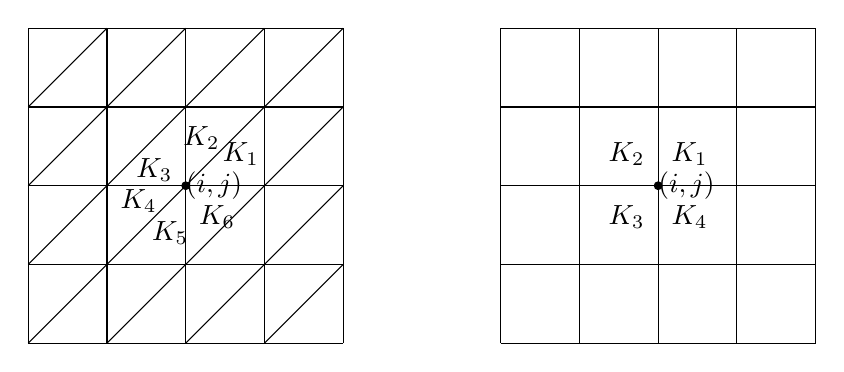
\begin{tikzpicture}[xscale=2,yscale=2]
%\tikzstyle{every node}=[font=\Large,scale=0.9]
\draw[-] (0,0) -- (2,0);
\draw[-] (0,0.5) -- (2,0.5);
\draw[-] (0,1) -- (2,1);
\draw[-] (0,1.5) -- (2,1.5);
\draw[-] (0,2) -- (2,2);

\draw[-] (0,0) -- (0,2);
\draw[-] (0.5,0) -- (0.5,2);
\draw[-] (1,0) -- (1,2);
\draw[-] (1.5,0) -- (1.5,2);
\draw[-] (2,0) -- (2,2);

\draw[-] (0,0) -- (2,2);
\draw[-] (0,0.5) -- (1.5,2);
\draw[-] (0,1) -- (1,2);
\draw[-] (0,1.5) -- (0.5,2);
\draw[-] (0.5,0) -- (2,1.5);
\draw[-] (1,0) -- (2,1);
\draw[-] (1.5,0) -- (2,0.5);

\node at (1.35,1.2) {$K_1$};
\node at (1.1,1.3) {$K_2$};
\node at (0.8,1.1) {$K_3$};
\node at (0.7,0.9) {$K_4$};
\node at (0.9,0.7) {$K_5$};
\node at (1.2,0.8) {$K_6$};

\node at (1.18, 1) {$(i,j)$};

\fill(1,1) circle(0.8pt);

\draw[-] (3,0) -- (5,0);
\draw[-] (3,0.5) -- (5,0.5);
\draw[-] (3,1) -- (5,1);
\draw[-] (3,1.5) -- (5,1.5);
\draw[-] (3,2) -- (5,2);

\draw[-] (3,0) -- (3,2);
\draw[-] (3.5,0) -- (3.5,2);
\draw[-] (4,0) -- (4,2);
\draw[-] (4.5,0) -- (4.5,2);
\draw[-] (5,0) -- (5,2);

\node at (4.2,1.2) {$K_1$};
\node at (3.8,1.2) {$K_2$};
\node at (3.8,0.8) {$K_3$};
\node at (4.2,0.8) {$K_4$};
\node at (4.18,1) {$(i,j)$};
\fill(4,1) circle(0.8pt);
\end{tikzpicture}
\end{center}
\end{figure}

For the piecewise linear finite element space, the nodal basis function $\phi^\ell_{i,j}$  associate with each $(x_i^\ell,y_j^\ell)$   
(satisfying \eqref{NodalBases-mul}) is given by 
\begin{equation}
  \label{LinearNodalBasis}
  \phi_{i,j}^\ell(x,y)=\left\{
  \begin{array}{ll}
\frac{x^\ell_{i+1}-x}{h}, & (x,y)\in K_1, \\
\frac{y^\ell_{j+1}-y}{h}, &(x,y)\in K_2,\\
\frac{x-x^\ell_{i-1}-(y-y^\ell_j)}{h}, &(x,y)\in K_3,\\
\frac{x-x^\ell_{i-1}}{h}, &(x,y)\in K_4,\\
\frac{y-y^\ell_{j-1}}{h}, &(x,y)\in K_5,\\
\frac{x^\ell_{i+1}-x+y-y^\ell_j}{h}, &(x,y)\in K_6\\
0, & \mbox{ elsewhere.} 
\end{array}
\right.
\end{equation}
shown in Fig. \ref{fig:nodallinear}.
\begin{figure}
\centering
\includegraphics[width=5.5cm,height=5cm]{figures/nodalbasis.pdf} 
\caption{\footnotesize{Nodal basis for linear element.}}
\label{fig:nodallinear}
\end{figure}

For bilinear element, it is easy to see that the nodal basis function $\phi^\ell_{i,j}$  associated with each $(x^\ell_i,y^\ell_j)$   
(satisfying \eqref{NodalBases-mul}) is given by 
\begin{equation}
  \label{BilinearNodalBasis}
  \phi^\ell_{i,j}(x,y)=\left\{
  \begin{array}{ll}
\frac{(x^\ell_{i+1}-x)(y^\ell_{j+1}-y)}{h^2}, \quad& (x,y)\in K_1, \\
\frac{(x-x^\ell_{i-1})(y^\ell_{j+1}-y)}{h^2}, \quad &(x,y)\in K_2,\\
\frac{(x-x^\ell_{i-1})(y-y^\ell_{j-1})}{h^2},\quad &(x,y)\in K_3,\\
\frac{(x^\ell_{i+1}-x)(y-y^\ell_{j-1})}{h^2},\quad &(x,y)\in K_4,\\
0 \quad & \mbox{ elsewhere.} 
\end{array}
\right.
\end{equation}


Associated with the above nodal basis functions $\phi^{\ell}_{i,j}(x,y)\subset \mathcal V_{\ell}$, 
we define the corresponding dual basis functions $\psi^{\ell}_{i,j}(x,y)\subset \mathcal V_{\ell}$ 
satisfying 
\begin{equation}
  \label{dual-basis}
(\psi^{\ell}_{i,j}(x,y), \phi^{\ell}_{p,q}(x,y))_{L^2(\Omega)}=\delta_{(i,j), (p,q)}.
\end{equation}
The existence of dual basis functions is obvious, but the exact expression of the dual basis functions are  
in general difficult to obtain. In fact, \eqref{dual-basis} is the only property that is needed in the application 
of dual basis. 

We write $\mathbf u_h(x,y)=\sum\limits_{i,j=1}^{n} u_{i,j}\phi_{i,j}(x,y), \mathbf v_h(x,y)=\sum\limits_{i,j=1}^{n} v_{i,j}\phi_{i,j}(x,y)$. 

\begin{lemma}
For bilinear functions, we have  
\begin{equation}\label{basis:plongation}
\begin{split}
\phi_{i,j}^{\ell+1}(x,y)&=\phi_{2i,2j}^{\ell}(x,y)+\frac{1}{2}\left(\phi_{2i-1,2j}^{\ell}(x,y)+\phi_{2i,2j-1}^{\ell}(x,y)
+\phi_{2i+1,2j}^{\ell}(x,y)+\phi_{2i,2j+1}^{\ell}(x,y)\right)\\
&+\frac{1}{4}\left(\phi_{2i-1,2j-1}^{\ell}(x,y)+\phi_{2i+1,2j-1}^{\ell}(x,y)
+\phi_{2i+1,2j+1}^{\ell}(x,y)+\phi_{2i-1,2j+1}^{\ell}(x,y)\right).
\end{split}
\end{equation}
For linear functions, we have  
\begin{equation}\label{basis:plongation2}
\begin{split}
\phi_{i,j}^{\ell+1}(x,y)&=\phi_{2i,2j}^{\ell}(x,y)
+\frac{1}{2}\left(\phi_{2i-1,2j-1}^{\ell}(x,y)+\phi_{2i+1,2j+1}^{\ell}(x,y)\right)\\
&+\frac{1}{2}\left(\phi_{2i-1,2j}^{\ell}(x,y)+\phi_{2i,2j-1}^{\ell}(x,y)
+\phi_{2i+1,2j}^{\ell}(x,y)+\phi_{2i,2j+1}^{\ell}(x,y)\right).
\end{split}
\end{equation}
\end{lemma}
Thus, for each $\mathbf v^{\boldsymbol {\ell}} \in \mathcal V_{\ell}, \mathbf f^{\boldsymbol {\ell}} \in \mathcal V'_{\ell}=\mathcal V_{\ell}$, we have 
\begin{equation}\label{expand}
\mathbf v^{\boldsymbol \ell}(x,y)=\sum_{i=1}^{m_\ell}\sum_{j=1}^{n_\ell}v^\ell_{i,j}\phi_{i,j}^\ell(x,y), 
~~ \mathbf f^{\boldsymbol \ell}(x,y)=\sum_{i=1}^{m_\ell}\sum_{j=1}^{n_\ell}f^\ell_{i,j}\psi_{i,j}^\ell(x,y),
\end{equation}
where
\begin{equation}
  \label{vf}
  v^\ell_{i,j}=\mathbf v^\ell(x_i^\ell,y_j^\ell),~~ f_{i,j}^\ell= (\mathbf f^\ell, \phi^\ell_{i,j})_{L^2(\Omega)}.
\end{equation}
Let us introduce the following tensors: 
\begin{equation}
  \label{v}
  v^\ell=(v^\ell_{i,j}),~~f^\ell=(f^\ell_{i,j}),~~\phi^\ell=(\phi^\ell_{i,j}),~~\psi^\ell=(\psi^\ell_{i,j}).
\end{equation}
The following identities obviously hold: 
$$
\mathbf v^\ell=(v^\ell, \phi^\ell)_{l^2},~~\mathbf f^\ell=(f^\ell, \psi^\ell)_{l^2},~~(\mathbf f^\ell,\mathbf v^\ell)_{L^2(\Omega)}=(f^\ell, v^\ell)_{l^2}.
$$

